\begin{savequote}[75mm]
I have done a terrible thing: I have postulated a particle that cannot be detected.
\qauthor{Wolfgang Pauli}
\end{savequote}

\chapter{Neutrino induced processes}
\label{sec:neu_dec}

In this chapter a very short description of the possible reactions detectable via tracking detectors and induced by neutrinos are described, as well as brief introduction to neutrino detection. 
The Author did not perform any physics analysis regarding the neutrinos but 
contributed to reconstruction algorithm described in the next chapter.

\section{Neutrino experiments}
Neutrino observation is one of the most challenging problems in modern particle physics.
Neutrino experiments come in many different shapes and sizes.
The notable examples of the extreme lengths that scientists come through pursuing the science of neutrinos include;

\begin{itemize}
\item Super-Kamiokande\cite{FUKUDA2003418} - a detector 1km deep underground, holding 50 220 tons of ultra-pure water
\item ANITA\cite{0503304} - radio pulse detector suspended on the helium balloon flying at the height of about 37,000 meters over the Antarctic
\item ICE-CUBE\cite{Abbasi_2009} - contains 5 160 optical sensors placed directly on the South Pole, 1,5 - 2,5 km deep inside the Antarctic ice sheet
\end{itemize}

\section{LARTPC detector}
LARTPC (Liquid Argon Time Projection Chamber) \cite{Rubbia:117852} detectors are a family of detectors developed from TPC detectors (Time Projection Chamber) \cite{osti_6545918}.
In general, such detectors consist of a volume of medium (radiator) between two plates (anode and cathode) that create an electric field.
When a particle travels through the detector's active volume, it excites the electrons, which interact with the electric field and move toward the collection plate (see Figure \ref{fig:lartpc-scheme}).
The TPC detectors used gas, and the LARTPC detector uses the same working principle, albeit the medium filling the volume is liquid argon.

\begin{figure}[ht]
\centering
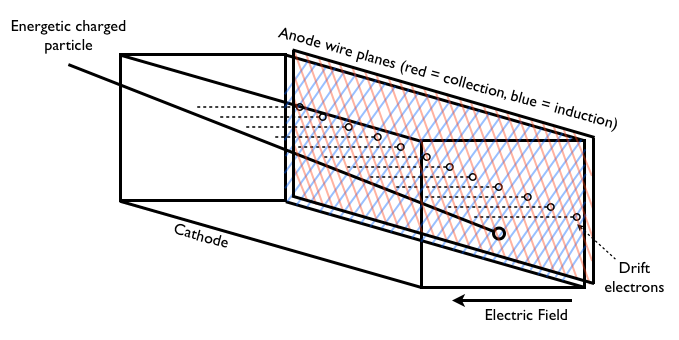
\includegraphics[width=0.95\textwidth]{figures/chapter6/RealSchematicTPC.png}
\caption[caption for LOF]{A diagram of LARTPC opration\footnotemark. }
\label{fig:lartpc-scheme}
\end{figure}
\footnotetext{ Source: \url{https://en.wikipedia.org/wiki/File:RealSchematicTPC.png}}

The argon is an excellent choice for the medium as it has high electron mobility (electrons are easily pulled along by the electric field) but low electronegativity (which means that the electrons will be less likely to be absorbed into the material).

The critical part of the design of the detector is its collection plates. There are two popular solutions of the LARTPC anode planes: pixel-based and wire-based. While the pixel-based approach is still mainly in development, the wire-based one is more popular and has been implemented in  MicroBoone, ICARUS, SBND, and the DUNE far detectors \cite{adams2020pilarnet}.
The anode for the wire-based design consists of multiple wire planes placed parallel to the cathode.
Each of the planes consists of multiple parallel wires.
The set of wire planes is kept at a bias voltage. Their electrostatic potential allows electrons to pass the first two planes undisturbed while inducing the signal. The electrons stop at the last plane called a collector.
Each of the first two planes (also called induction planes) has a unique orientation of the wires.
This orientation allows for a reconstruction of the 2D signal ( Figure \ref{fig:lartpc-grids}).
Additionally, a 3D reconstruction is possible to obtain by calculating the distance travelled by the electrons, using the 2D and the constant flow rate of the electrons.
This requires trigger information, which can either come from the particle source or can be achieved using the scintillation effect (light flash) of the argon.
The trigger information provides the timing information about the event \cite{microboone}.

\begin{figure}[H]
\centering
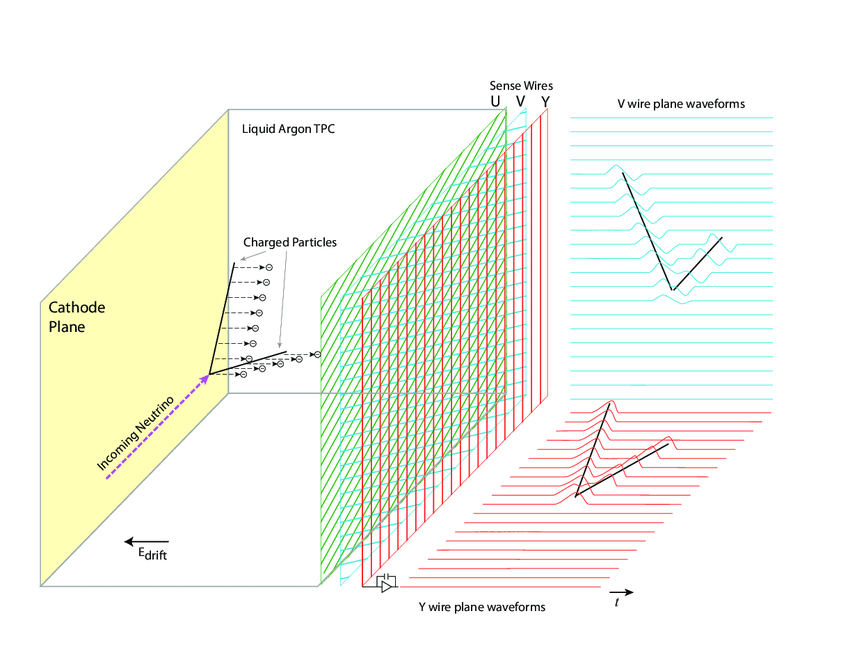
\includegraphics[width=.6\textwidth]{figures/chapter6/Operational-principle-of-the-MicroBooNE-LArTPC.png}
\caption{A diagram of LARTPC planes \cite{microboone}}
\label{fig:lartpc-grids}
\end{figure}

\section{Neutrino production and observation}

In order to paint a better picture of the nature of the neutrino detection, this section depcits some of the interactions in physics that involve neutrino.
Neutrinos are notorious for their elusiveness. Their only known interaction with matter is through the weak force.
One of their most popular interaction is in \textbf{beta decay}, otherwise the neutrinos in the range of medium and higher energies interact via: \textbf{Elastic and Quasielastic scattering}, \textbf{Deep inelastic scattering} and \textbf{Resonance production}.

\begin{figure}[H]
\centering
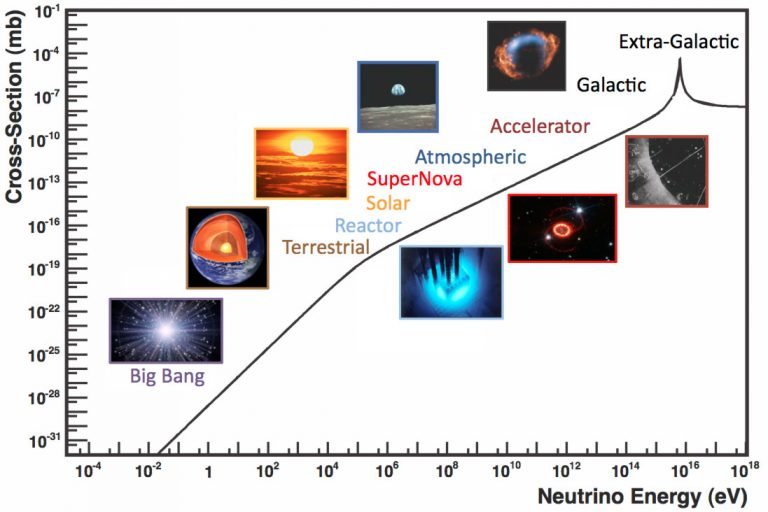
\includegraphics[width=0.6\textwidth]{figures/chapter6/neutrino-energy-scale.jpg}
\caption{Neutrino energy scale \cite{RevModPhys.84.1307}}
\label{fig:neutrino-energy}
\end{figure}

\subsection{Beta-decay}

The simplest processes that involves neutrinos are $\Beta^{-}$ and  $\Beta^{+}$ decays.
The common examples of these processes are $n \rightarrow p + e^{-}+\bar{\nu}_e$ and $n \rightarrow p + e^{+}+\nu_e$ respectively, which on the quark level can be expressed as $u \rightarrow d + e^{-}+\bar{\nu_e}$ (Fig \ref{plot:beta_m}) and $d \rightarrow u + e^{+}+\nu_e$ (Fig \ref{plot:beta_p}).

\begin{figure}[H]
\centering
\begin{subfigure}[b]{0.35\textwidth}
    \centering
    
\includegraphics[width=\linewidth]{figures/chapter6/768px-Beta_Negative_Decay.svg.png}
% \caption{}
\caption{Beta minus}
    \label{plot:beta_m}
  \end{subfigure}
\begin{subfigure}[b]{0.35\textwidth}
    \centering
    
\includegraphics[width=\linewidth]{figures/chapter6/768px-Electron_Capture_Decay.svg.png}
\caption{Beta plus}
% \caption{}
   \label{plot:beta_p}
  \end{subfigure}
  \caption[Beta decay]{Two types of beta decays involving neutrino\footnotemark. }

    \label{plot:beta_decays}
\end{figure}
\footnotetext{ Image source: \url{https://commons.wikimedia.org/wiki/File:Beta_Negative_Decay.svg} and \url{https://commons.wikimedia.org/wiki/File:Electron_Capture_Decay.svg}}


\subsection{Medium and higher energy interactions}


The most interesting range of energies, defined arbitrarily, for neutrinos spans from medium ($0.1 GeV$) to high ($1TeV$) values.
As previously stated, neutrinos only interact with the matter through weak interaction.
This is why the neutrino is not directly detectable, but instead, detectors rely on secondary particles for evidence of neutrinos.
Multiple probable processes can produce observable particles (see Figure \ref{plot:neutrino_cross_section}); I will introduce some more probable ones in this subsection.

\begin{figure}[H]
\centering
\begin{subfigure}[b]{0.45\textwidth}
    \centering
    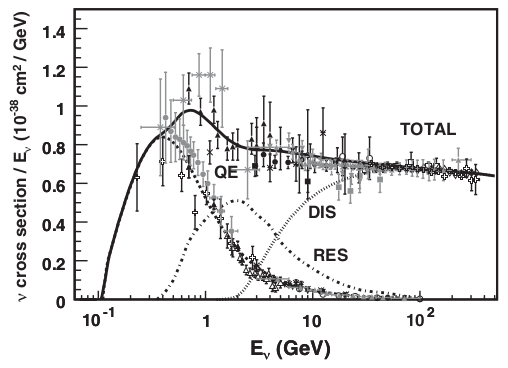
\includegraphics[width=\linewidth]{figures/chapter6/neutrino_cross_mid.png}
% \caption{}
\caption{Neutrino}
    \label{plot:cross_neu}
  \end{subfigure}
\begin{subfigure}[b]{0.45\textwidth}
    \centering
    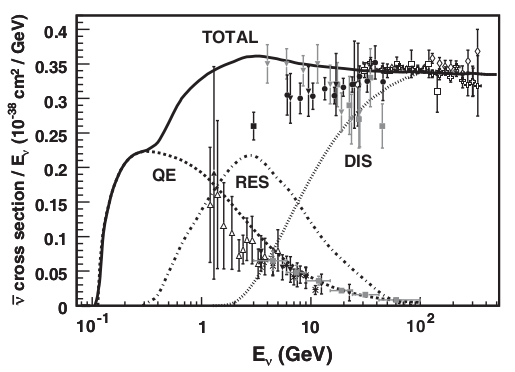
\includegraphics[width=\linewidth]{figures/chapter6/antineutrino_cross_mid.png}
\caption{Antineutrino}
% \caption{}
   \label{plot:cross_anti}
  \end{subfigure}
  \caption[neutrino interactions]{Neutrino (A) and Antineutrino cross-section in GeV section with contribution from different processes. \cite{RevModPhys.84.1307}}

    \label{plot:neutrino_cross_section}
\end{figure}

\subsubsection{Elastic and Quasielastic scattering}
\label{sec:QE}

Neutrinos can elastically interact with the atom's nucleus what leads to their excitation and possible emission of nucleon.
It is as simple as that in the case of the neutral current elastic scattering. Neutrino interacts with the nucleus and frees a proton or neutron, which can later interact with matter more easily.
In the case of the charged current quasi-elastic (CCQE) interaction, it changes the nucleon and emits a lepton.
For the free nucleon interaction it is: $\nu + n \rightarrow l^{-}+p$ and $\bar{\nu} + p \rightarrow l^{+}+n$ where $l$ stands for lepton.
Fig \ref{plot:CCQE} depicts exemplary CCQE scattering. It is important to note that this interaction both releases a nucleon and produces charged particle.
The quasi-elastic scattering is the most popular interaction in the medium range of energies.

\begin{figure}[H]
\centering
\begin{subfigure}[b]{0.28\textwidth}
    \centering
    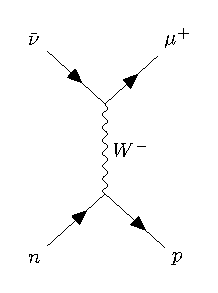
\includegraphics[width=\linewidth]{figures/assets/feyman_graphs/CCQE.pdf}
% \caption{}
\caption{Beta minus}
    \label{plot:ccqe_p}
  \end{subfigure}
\begin{subfigure}[b]{0.28\textwidth}
    \centering
    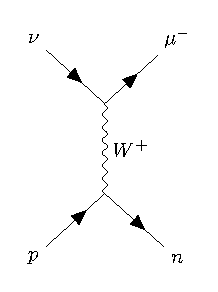
\includegraphics[width=\linewidth]{figures/assets/feyman_graphs/CCQE-anti.pdf}
\caption{Beta plus}
% \caption{}
   \label{plot:ccqe_m}
  \end{subfigure}
  \caption[Beta decay]{\@TODO  }

    \label{plot:CCQE}
\end{figure}


  \subsubsection{Deep inelastic scattering}
\label{sec:DIS}

In deep inelastic scattering, neutrino scatters off on a quark coming from a nucleon.
The scattering is conveyed by a virtual boson (W or Z). In cases of a CC produces a $\mu$ or $\mu^{-}$.
The NC process doesn't produce additional charged particles.
The examples below present the case with the $\nu_{\mu}$, but other types of neutrinos are also allowed in deep inelastic scattering.
Some of the possible processes of DIS:

\begin{align*}
\nu_{\mu} N \rightarrow \mu^{-}X \\
\bar{\nu}_{\mu} N \rightarrow \mu^{+}X \\
\nu_{\mu} N \rightarrow \nu_{\mu}X \\
\bar{\nu}_{\mu} N \rightarrow \bar{\nu}_{\mu}X
\end{align*}

\begin{figure}[H]
\centering
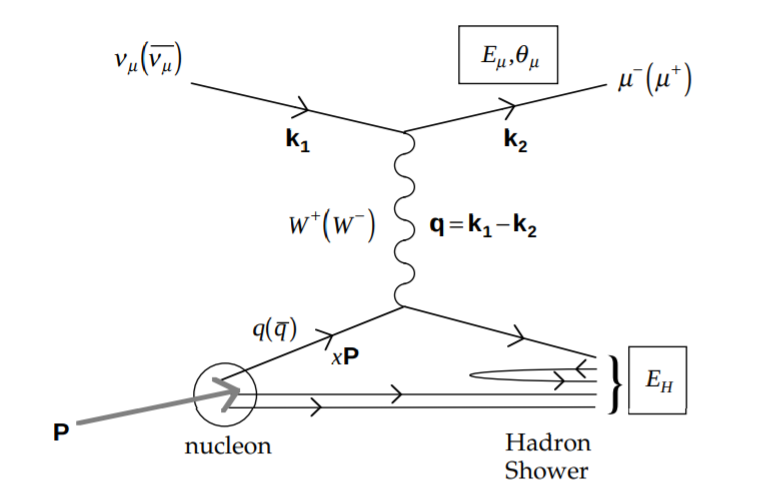
\includegraphics[width=0.6\textwidth]{figures/chapter6/deepinelastic.png}
\caption{A diagram of deep inelastic interaction of a neutrino with a neutron (charged current)\cite{Conrad_1998}.}
\label{fig:deep-inelastic}
\end{figure}

% Medium and high energy processes
% https://arxiv.org/abs/1305.7513
% https://indico.cern.ch/event/819261/contributions/3423332/attachments/1885005/3106900/lecture2_betancourt_2019.pdf
\subsubsection{Resonance production}
\label{sec:RES}

With enough energy, neutrinos can cause the excitation of a nucleon. This excited state produces a baryon resonance along with a lepton, and then the resonance quickly decays into a nucleon and an accompanied meson:

\begin{align*}
\nu_{\mu} N \rightarrow \mu^{-}N* \\
N* \rightarrow \pi N
\end{align*}

  Other decays modes are also possible but less probable. The most common pion production is possible in this interaction. For $\nu_{\mu}$ and $p, n$ targets, there are seven possible resonant single pion reaction channels (seven each for neutrino and antineutrino). In those channels, only two of them do not produce a charged particle.


\section{Ultra high energy neutrinos}

The neutrinos of the ultra high energy are impossible to be produced on earth (yet), so they are searched in the cosmic radiation. All of the experiments mentioned in the list Section \ref{sec:neu_dec}, are focused on registering ultra high energy neutrinos from space. The task is problematic not only because of the small cross-section of the interaction of a neutrino with the matter but also because of the other types of radiation that can obscure the discoveries. This is why they need a very thick shielding (Super Kamiokande and ICE-CUBE).
Due to the rarity, ultra high energy neutrinos are one of the least experimentally researched branches of particle physics and thus are worthy of mentioning here.


\section{Summary}

This chapter introduces reader to the LARTPC detector as well as basic processes in neutrino physics.

Although the neutrinos themselves are limited to only weak interactions, after the deposition of the energy, a vast array of mostly charged particles can either be produced, excited or use the deposited energy to create a further chain of reaction.
The selected processes depicted in Sec. \ref{sec:QE}-\ref{sec:RES}, provide a short glance at the possibilities.
It is worth noting that although there exist many channels of interaction for the neutrino, the cross-sections are very small compared to other branches of physics.

This theoritical introduction is important in consideration of the next chapter, where I present the algorithm for the LARTPC detector.

%%% Local Variables:
%%% mode: latex
%%% TeX-engine: xetex
%%% TeX-command-extra-options: "-shell-escape"
%%% TeX-master: "../dissertation"
%%% End:
